\documentclass[10pt,a4paper]{report}
\usepackage{fontspec}
\defaultfontfeatures{Mapping=tex-text}
\usepackage{xunicode}
\usepackage{xltxtra}
%\setmainfont{???}
\usepackage{polyglossia}
\setdefaultlanguage{spanish}
\usepackage{amsmath}
\usepackage{amsfonts}
\usepackage{amssymb}
\usepackage{graphicx}
\usepackage[left=2cm,right=2cm,top=2cm,bottom=2cm]{geometry}

\title{\textbf{INFORME FINAL DE ACTIVIDADES DE SERVICIO SOCIAL.}\\\textit{Laboratorio de Sistemas Complejos - FING}\\
\includegraphics[scale=0.2]{logo_fing_uach_bn.png}}
\author{Natividad Oswaldo Pérez Medina.\\Ing. Matemática - 357417}


\begin{document}
\maketitle
\newpage
\section{Introducción}
El presente informe describe las actividades realizadas durante el servicio social en el Laboratorio de Sistemas Complejos de la Facultad de Ingeniería de la Universidad Autónoma de Chihuahua. El proyecto en el que participé se enfoca en el desarrollo de un modelo predictivo para estimar la probabilidad de deserción estudiantil, utilizando datos académicos, demográficos y sociales.

\bigskip

Dicho modelo parte de la premisa de que el rendimiento académico y el contexto socioeconómico de los estudiantes influyen en su permanencia escolar. En particular, se utilizan los datos históricos proporcionados por la UACH en el momento de la inscripción y a lo largo del historial académico de cada estudiante, así como indicadores oficiales del grado de marginación de sus localidades de residencia. Este enfoque permite identificar con mayor precisión a aquellos estudiantes en situación de riesgo, a fin de enfocar mejor los programas de apoyo institucional.
\section{Justificación}
El desarrollo de este proyecto responde a la necesidad social y académica de atender la problemática de la deserción escolar desde una perspectiva científica y preventiva. Para los estudiantes que realizamos nuestro servicio social en este entorno, el proyecto representa una oportunidad valiosa de aplicar conocimientos matemáticos en un contexto real y profesional, fortaleciendo así nuestras competencias técnicas y analíticas.

\bigskip

Asimismo, este tipo de experiencias permite consolidar habilidades que son fundamentales para el ejercicio profesional de un matemático: análisis de datos, estructuración de código, trabajo colaborativo y documentación técnica. El proyecto no solo contribuye al fortalecimiento institucional, sino que también abre caminos hacia la investigación aplicada y el desarrollo de herramientas con impacto social.

\section{Objetivos}
\begin{itemize}
    \item Cumplir con el compromiso universitario de retribuir a la sociedad mediante el servicio social.
    \item Aplicar conocimientos matemáticos y computacionales en un entorno de investigación científica.
    \item Colaborar en el desarrollo y mejora de herramientas destinadas a predecir la deserción escolar.
    \item Documentar y optimizar procesos dentro del proyecto, fomentando la mejora continua del mismo.
    \item Fortalecer habilidades profesionales tales como el trabajo en equipo, la documentación técnica y la comunicación efectiva.
\end{itemize}
\bigskip
\begin{center}
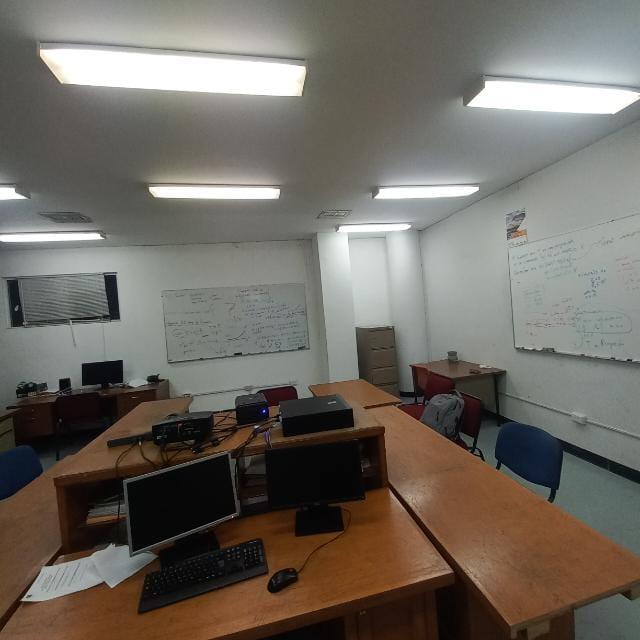
\includegraphics[scale=0.3]{5df11f7e-c191-4aee-8b7a-c76222a9ed0f.jpeg}\\
\textbf{Figura 1:} Espacio donde se desarrolló el servicio social.
\end{center}
 

\newpage

\section{Metodología}

El proyecto se estructura en un pipeline automatizado que permite transformar grandes volúmenes de datos académicos y sociales en insumos procesables por modelos de predicción de deserción. Este flujo de trabajo está compuesto por varias etapas interconectadas, representadas en un diagrama general que organizamos durante el desarrollo del proyecto. A continuación, se detallan los principales componentes de dicha metodología, de acuerdo con el diagrama:

\subsection{Obtención y separación inicial de datos}

El proceso inicia con una base de datos en formato .csv que contiene información académica completa de una generación específica (por ejemplo, "2023-2 completo"). Esta base se somete a una fase de filtrado mediante un módulo denominado "Básico", el cual organiza los datos por semestre (/Sem) y separa los campos relevantes:

\begin{itemize}
\item Calificaciones
\item Datos generales
\item Identificadores
\end{itemize} 

Esta separación facilita el manejo de los datos y su posterior integración en diferentes etapas del modelo, además de permitir una depuración más precisa.

\subsection{Generación de bloques por semestre}

Los datos separados por semestre son dirigidos al componente ''generador-georef'', el cual se encarga de crear directorios específicos por grupo y generar un archivo intermedio llamado Direcc-data.csv que contiene las direcciones académicas por alumno, además de su georeferencia (laltitud y longitud recolectada con Google Maps). Este archivo es esencial para mapear las rutas hacia archivos con información más detallada por estudiante.

\subsection{Distribución y estructuración para el modelo}

Una vez creados los directorios y bloques de información, los datos son distribuidos en carpetas organizadas por estudiante y semestre. Se generan archivos intermedios como BaseN-GMN.csv, los cuales contienen promedios, conteos y calificaciones procesadas y estandarizadas.

\bigskip

En paralelo, se ejecutan scripts que asignan los grados de marginación a cada estudiante, utilizando como referencia su ubicación geográfica en el estado de Chihuahua.

\subsection{Integración de información y empaquetado}

Con los datos organizados, se realiza una integración en un archivo consolidado llamado final-n.csv. Este archivo agrupa toda la información necesaria por estudiante para alimentar el modelo de predicción. Esta etapa también implica copiar ciertos bloques y concatenar archivos para lograr uniformidad en la estructura.

\subsection{Interfaz gráfica y ejecutables}

Para facilitar la interacción con el sistema, se desarrollaron dos ejecutables principales con interfaz gráfica:

\begin{itemize}
\item \textbf{GUIBOTLINUX:} Automatiza el flujo de procesamiento y limpieza desde los archivos de entrada hasta la generación de salidas listas para el modelo.

\item \textbf{GUIverif}: Permite verificar la integridad y el contenido de las bases generadas, así como exportar archivos clave como:
\begin{itemize}
\item Direcc.geo.csv (con coordenadas geográficas)
\item Direcc.open.csv (con estructura normalizada de entrada)
\item Direcc.concent.csv (concentrado final por estudiante)
\end{itemize}
\end{itemize}

Ambos ejecutables fueron construidos en Python, utilizando la biblioteca CustomTkinter para facilitar su uso por parte de investigadores y futuros colaboradores.


\subsection{Recursos tecnológicos}

Las actividades se desarrollaron en estaciones de trabajo con sistema operativo Linux. Se utilizaron entornos locales y remotos (Google Colaboratory) para la ejecución de scripts, combinando programación en Python con manejo de estructuras de carpetas y archivos en disco. Además, se utilizaron herramientas como pandas, NumPy, y bibliotecas para empaquetado de scripts en ejecutables.

\section{Resultados}

\subsection{Proyecto de Carga y Procesamiento de Datos Académicos y Grados de Marginación}

Uno de los principales logros durante mi servicio social fue el desarrollo e integración de un ejecutable que permite automatizar el proceso de análisis y preparación de datos para el modelo de predicción de deserción. Este ejecutable, resultado de la integración de códigos propios y de otros colaboradores, permite calcular y consolidar en un solo archivo los siguientes elementos por estudiante:

\begin{itemize}
\item Datos académicos de inscripción.
\item Historial de promedios semestrales.
\item Índices de avance académico.
\item Nivel de marginación territorial.
\end{itemize}

El archivo generado se convierte en una base de datos limpia y estandarizada que sirve como insumo para las siguientes etapas del modelo. Además, desarrollé una interfaz gráfica que facilita la interacción con dicho ejecutable, haciendo más accesible su uso para futuros colaboradores o responsables del sistema.

\subsection{Predicciones 2024-2}

Durante mi periodo de servicio social, se generaron las primeras predicciones correspondientes al semestre 2024-2, aplicadas sobre la lista de alumnos registrados en la base de datos institucional de la UACH.

\bigskip

El modelo, una vez alimentado con la base procesada por el ejecutable desarrollado, asignó a cada estudiante un valor numérico entre 0 y 1, el cual representa la probabilidad estimada de deserción escolar. Estos valores permiten identificar a los estudiantes en situación de riesgo y orientar mejor las políticas de atención prioritaria por parte de la universidad.

\subsection{Predicciones 2025-1}

Asimismo, se llevaron a cabo las predicciones correspondientes al semestre 2025-1, aplicando el mismo procedimiento sobre la nueva lista de estudiantes inscritos. Este segundo ejercicio permitió verificar la estabilidad del modelo predictivo, además de reforzar los criterios de comparación entre cohortes y la evolución de los factores que inciden en la deserción.

\bigskip

Los resultados fueron registrados y almacenados en archivos específicos, listos para análisis por parte del equipo de investigación y para su posible uso en intervenciones institucionales.

\subsection{Actividades de Divulgación Científica y Vinculación con AMCCh}

De manera paralela al trabajo técnico, participé en actividades de divulgación científica en colaboración con la Academia de Matemáticas y Ciencias de Chihuahua (AMCCh). Estas actividades tenían como objetivo acercar a estudiantes de nivel medio superior a herramientas prácticas de programación, ciencia de datos y pensamiento científico.

\bigskip

En una primera sesión, once alumnos de la Academia visitaron el laboratorio, donde participaron en ejercicios prácticos relacionados con el análisis de datos y lógica computacional. Posteriormente, nosotros acudimos a las instalaciones de la AMCCh, donde realizamos una segunda jornada de trabajo con enfoque en experimentación y participación activa, reforzando así los conceptos vistos en su ciclo escolar. Estas actividades fortalecieron el vínculo entre la universidad y los jóvenes talentos interesados en las ciencias exactas.

\newpage

\section{Conclusiones}

\begin{enumerate}
\item Realizar el servicio social en el Laboratorio de Sistemas Complejos fue una experiencia enriquecedora que me permitió trabajar en un entorno profesional alineado con mi formación como estudiante de matemáticas. A través del desarrollo de herramientas técnicas y la colaboración en un proyecto de impacto social, pude visualizar de manera concreta el papel que puede desempeñar un matemático en contextos reales y complejos.
\item Esta experiencia me brindó una base sólida para profundizar en mis intereses profesionales, influyendo directamente en la definición de mi tema de tesis y orientándome hacia futuras metas académicas, como lo es una maestría en ciencias de datos o computación. Además, me permitió consolidar habilidades en programación, diseño de interfaces y documentación técnica, aspectos clave para cualquier carrera profesional en el área científico-tecnológica.
\item El proyecto representa una oportunidad única para estudiantes interesados en aplicar la matemática a problemas reales mediante el análisis de datos, y constituye un ejemplo de cómo el servicio social puede ser una plataforma de formación profesional y académica con impacto tangible.

\end{enumerate}



\section{Recomendaciones}
\subsection{A la Unidad Receptora}

De manera personal, recomendaría que, debido a la constante afluencia de alumnos en el laboratorio, se implementen carteles visibles que indiquen el uso adecuado de las instalaciones. Considero que sería útil contar con señalización que recuerde prácticas como mantener limpios los pizarrones al finalizar la jornada, apagar los equipos después de su uso, y respetar el espacio compartido. Este tipo de recordatorios ayudaría a fomentar una mejor convivencia y a mantener el orden dentro del laboratorio, especialmente en horarios con alta actividad.

\subsection{A la Unidad Central de Servicio Social}

Desde mi experiencia, sugeriría que se elabore un documento oficial, claro y completo, que explique paso a paso todo el proceso del servicio social: desde cómo registrarse, los formatos requeridos, tiempos de entrega, hasta el proceso final de liberación. Sería ideal que este documento estuviera disponible directamente en el sistema SEGA, para que cualquier estudiante pueda consultarlo sin necesidad de buscar respuestas en distintos lugares. En mi caso particular, no tuve mayores complicaciones, pero considero que una guía consolidada evitaría muchas confusiones comunes entre los compañeros.

\subsection{A la Unidad de Servicio Social}

En lo personal, no tengo recomendaciones específicas para esta unidad, ya que en mi experiencia todo el proceso fue claro y bien gestionado. El acompañamiento, la atención y los tiempos de respuesta fueron adecuados. Mi sugerencia sería simplemente que se mantenga esa misma línea de trabajo, con el mismo nivel de atención y organización que tuve la oportunidad de experimentar durante mi servicio social.

\section{Evidencias}
\centering
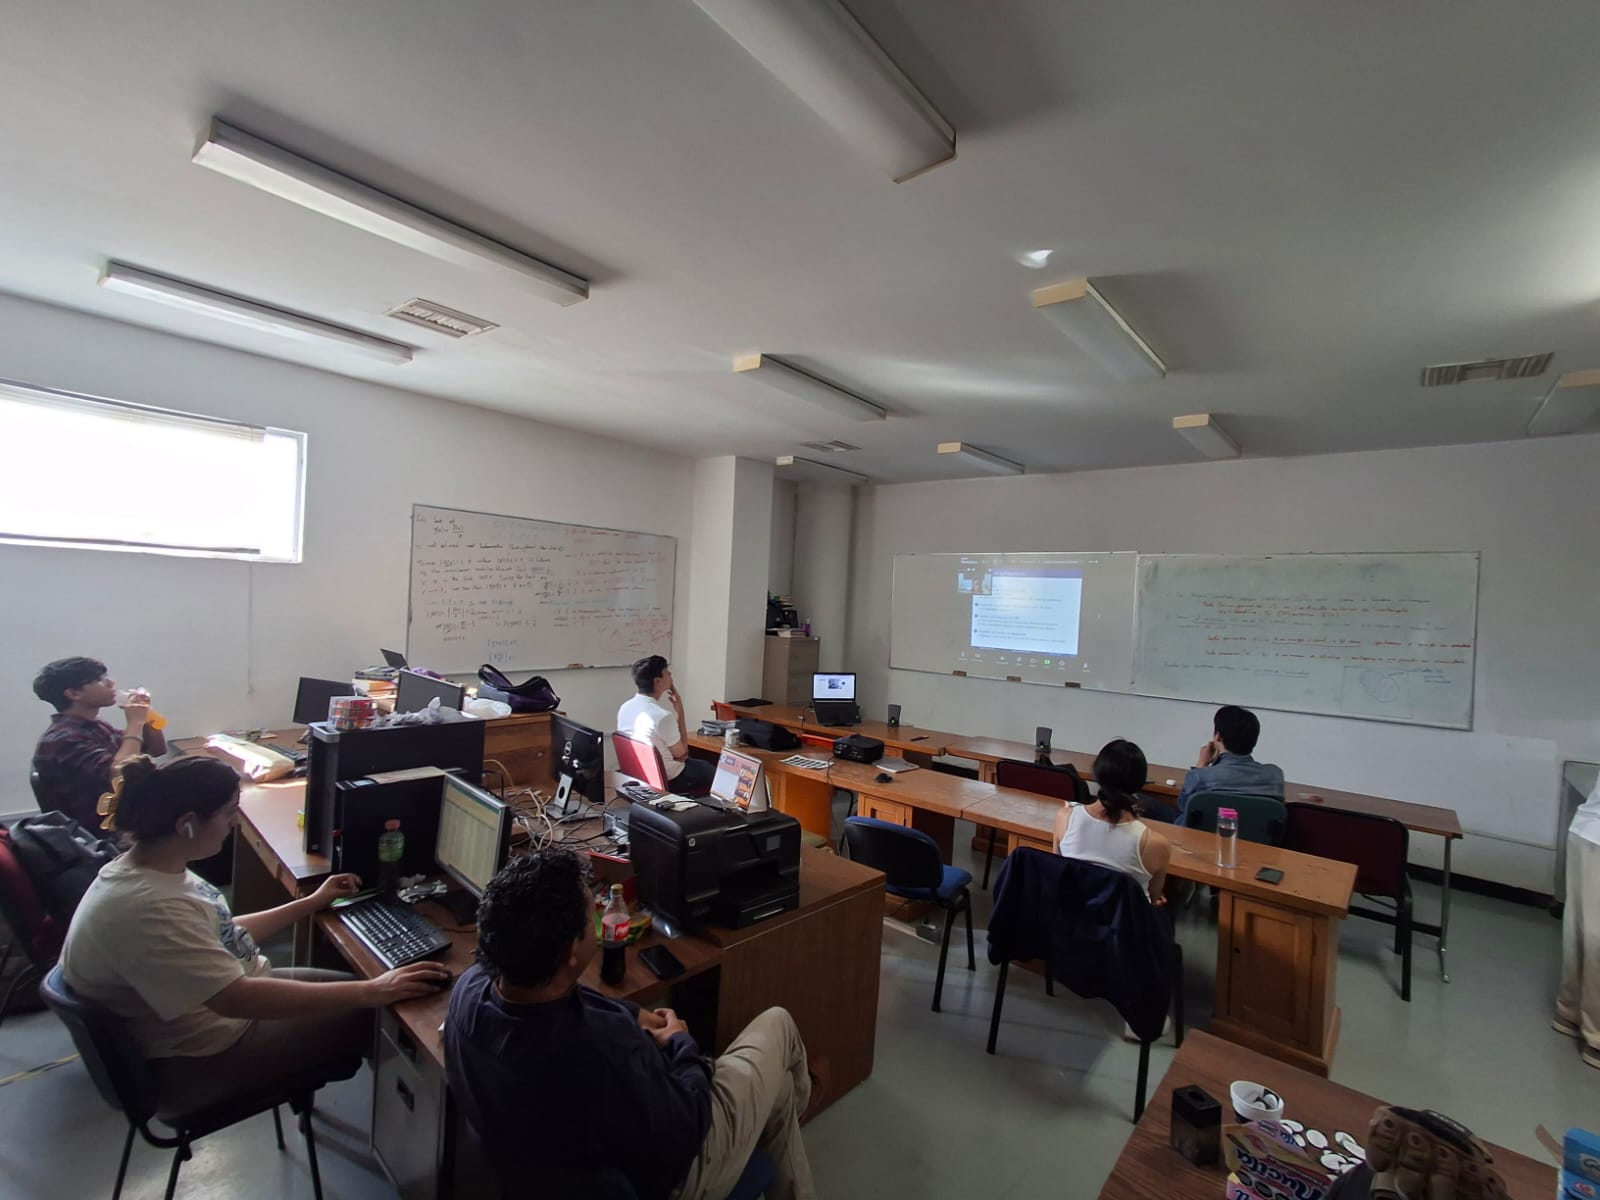
\includegraphics[scale=0.2]{5cc66181-2a51-4b15-ab18-15ef2e99302b.jpeg} \\
\bigskip
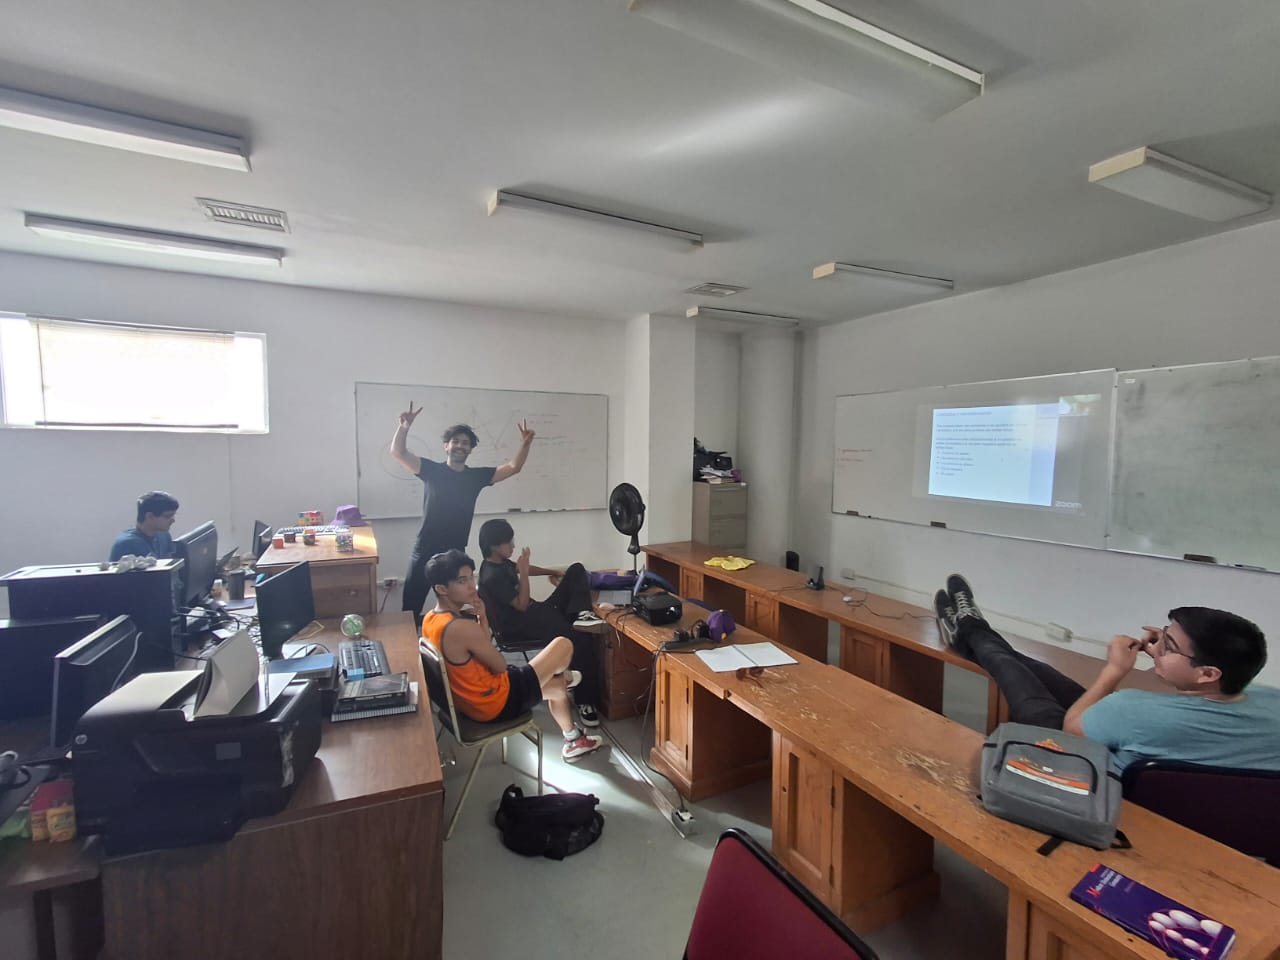
\includegraphics[scale=0.3]{05108b8e-31a0-47e7-b65a-0e2036ec6b9b.jpeg} 

\end{document}